%\algnewcommand{\IfNDebug}[1]{#1}
%\algnewcommand{\IfNDebug}[1]{}

\chapter{McSplit-SI: An algorithm for the induced subgraph isomorphism problem
optimised for large, sparse graphs}
\label{c:mcsplit-si}

\section{Introduction}

In the induced subgraph isomorphism problem, we seek to find an induced copy of pattern graph $G$ in target graph $H$. This is special case of the decision version of maximum common induced subgraph in which we require the common subgraph to contain all of graph $G$'s vertices.

The \McSplit\ algorithm may be trivially modified to solve the induced subgraph isomorphism problem. Rather than calculating an upper bound at each search node, we simply backtrack when the $G$-set of any label class is larger than the corresponding $H$-set, since by the pigeonhole principle this implies that we cannot map each pattern-graph vertex to a target-graph vertex.

While \McSplit\ is well suited to the small (tens of vertices), relatively dense graphs that are typical of maximum common subgraph instances, it has two disadvantages for large (hundreds or thousands of vertices), sparse graphs that appear in benchmark instances for subgraph isomorphism.  The first disadvantage relates to space: $b(n_G^2 + n_H^2)$ space is needed to store the adjacency matrices, where $b$ is the memory size of a boolean variable.\footnote{We could switch to a more space-efficient representation such as hash-sets of neighbours which would still permit constant-time adjacency tests in the algorithm's partitioning step, but this would slow down the algorithm significantly.}  The second disadvantage relates to time: during the partitioning step, the \McSplit\ algorithm iterates over all of the vertices in each label class, which often requires checking close to $n_G + n_H$ adjacency-matrix elements each time the partitioning procedure is carried out.

\Cref{figure:si-targets-n-density} shows vertex count and density for the target graphs of a random subset of the benchmark instances
that we will use in this chapter.  Of the entire benchmark set, $76\%$ of pattern graphs have density less than $0.01$.  Thus, it would
greatly improve our \McSplit\ algorithm for subgraph isomorphism if we could reduce the time complexity of the partitioning
step from $O(n_G + n_H)$ to $O(|N(v)| + |N(w)|)$, where $(v,w)$ is the most-recently made mapping of a pattern vertex to a target
vertex.  In this chapter we introduce this improved algorithm, which we call \McSplit-SI.

\begin{figure}[h!]
    \centering
    \includegraphics*[width=0.6\textwidth]{14b-mcsplit-induced-si/density-chart/plots/n-density}
    \caption{Number of vertices and density (log scale) of a sample of 1000 target graphs from the benchmark set
    of $14,621$ subgraph isomorphism instances.}
    \label{figure:si-targets-n-density}
\end{figure}

\section{The label class object}

In the \McSplit\ algorithm, the label class objects at each level of the search tree are stored
contiguously in an array, and each object requires only four indices or pointers: to the start and
end of the $G$-set and the $H$-set.  To enable partitioning in $O(|N(v)| + |N(w)|)$ time, \McSplit-SI
requires a more elaborate object type, and stores the objects in a doubly-linked list which is modified
when partitioning domains and restored on backtracking.

\Cref{tab:mcsplit-si-object} lists the member variables of a label class object.  Rather than
using an external doubly-linked containing label class objects, we store the $\AlgVar{prev}$
and $\AlgVar{next}$ pointers within each object; thus our list of label classes is an ``intrusive
linked list''.  These pointers are useful not only for iterating over the list but also
for restoring deleted elements when backtracking, as we will discuss later in the chapter.

The first four members of the object play the same role as the four indices used in \McSplit's
simpler label class object: they point to the ranges in the permuations of $V(G)$ and $V(H)$ that
contain the $G$-set and $H$-set.

\FloatBarrier

\begin{table}[h!]
\centering
\footnotesize
 \begin{tabular}{p{0.13\linewidth} p{0.2\linewidth} p{0.5\linewidth}}
 \toprule
    Name & Type & Description \\ [0.5ex]
 \midrule
    $s_G$ & Pointer to Integer & Pointer to the first vertex of the $G$-set\\
    \rule{0pt}{2.3ex}$e_G$ & Pointer to Integer & Pointer to one element past the last vertex of the $G$-set\\
    \rule{0pt}{2.3ex}$s_H$ & Pointer to Integer & Pointer to the first vertex of the $H$-set\\
    \rule{0pt}{2.3ex}$e_H$ & Pointer to Integer & Pointer to one element past the last vertex of the $H$-set\\
    \rule{0pt}{2.3ex}$\AlgVar{a}$ & Boolean & ``active'': Is this label class in the doubly linked list? \\
    \rule{0pt}{2.3ex}$\AlgVar{s}$ & Boolean & ``splitting'': Is this label class being split? \\
    \rule{0pt}{2.3ex}$\AlgVar{prev}$ & Pointer to Label Class & The previous label class in the doubly-linked list of all label classes \\
    \rule{0pt}{2.3ex}$\AlgVar{next}$ & Pointer to Label Class & The next label class in the doubly-linked list of all label classes \\
%%      \rule{0pt}{2.3ex}$\AlgVar{next\_deleted}$ & Pointer to Label Class & The next label class in a singly-linked list of deleted label classes (to be restored on backtracking)\\
%%      \rule{0pt}{2.3ex}$\AlgVar{next\_split}$ & Pointer to Label Class & The next label class in a singly-linked list of split label classes (to be merged on backtracking)\\
%%  \midrule
%%     $a_G$ & Integer & Number of vertices adjacent to $v$ \\
%%     $a_H$ & Integer & Number of vertices adjacent to $w$ \\
%%      \rule{0pt}{2.3ex}$\AlgVar{next\_free}$ & Pointer to Label Class & The next label class in the free list \\
 \bottomrule
\end{tabular}
\caption{The member variables of \McSplit-SI label class object}
\label{tab:mcsplit-si-object}
\end{table}

\FloatBarrier

Initially, the doubly-linked list of label classes contains a single element representing
all vertices of graphs $G$ and $H$.  \Cref{figure:si-data-structures} shows the data structures
after making the assignment $(1,a)$ in our example graphs $G$ and $H$ from \Cref{c:mcsplit-i-undirected}.

The top and bottom rows of the diagram contain the final element of our data structure, which we
have not yet described.  We have two arrays, $\AlgVar{Gptrs}$ and $\AlgVar{Hptrs}$, which contain
an object for each vertex $v$ of $G$ and $H$ respectively.  Each object contains two pointers.
The first points to the position in the permutation at which $v$ appears, and the second points
to the label class containing $v$.  The arrays $\AlgVar{Gptrs}$ and $\AlgVar{Hptrs}$ will allow
us to carry out the partitioning step without iterating over the vertices in each label class.

\begin{figure}[h!]
    \centering
    $G=$\tikz {
        \graph [nodes={draw, circle, minimum width=.55cm, inner sep=1pt}, circular placement, radius=0.95cm,
                clockwise=5] {
                    1,2,3,4,5;
            1--4; 1--5; 2--3; 2--5; 3--5;
        };
    }
    \qquad\qquad
    $H=$\tikz {
        \graph [nodes={draw, circle, minimum width=.55cm, inner sep=1pt}, circular placement, radius=0.95cm,
                clockwise=6, phase=60] {
                    a,b,c,d,e,f;
            a--b; a--c; a--e; b--d; b--f; c--d; c--e; c--f; d--f; e--f;
        };
    }
    \includegraphics*[width=0.9\textwidth]{14b-mcsplit-induced-si/figs/data-structure-step-1}
    \caption{The data structures of \McSplit-SI after assigning vertex $1$ to vertex $a$.
        Circles represent pointers; hollow circles are null pointers.  The middle row shows
        the doubly-linked list of label classes.  Shown immediately above and below this are the
        permutations of $V(G)$ and $V(H)$, stored as arrays.  The top and bottom rows
        show the arrays $\AlgVar{Gptrs}$ and $\AlgVar{Hptrs}$.  Each element of these arrays
        corresponds to a vertex $v$ of $G$ or $H$, and points to the position of $v$
        the permutation and to the label class containing $v$.  To reduce clutter in the diagram,
        the label class pointers are shown pointing to a rectangle of the same colour as the
        label class.}
    \label{figure:si-data-structures}
\end{figure}

\section{The partitioning algorithm}

When making a tentative assignment of vertex $v$ to vertex $w$, we perform the same steps
as the basic \McSplit\ algorithm: swap $v$ and $w$ to the
end of their label class in the $V_G$ and $V_H$ arrays, and decrement the end pointers
of that label class.  The \McSplit-SI algorithm requires additional (constant time)
steps to maintain the invariants of
the $\AlgVar{Gptrs}$ and $\AlgVar{Hptrs}$ arrays: set the label-class pointers of
$\AlgVar{Gptrs}[v]$ and $\AlgVar{Hptrs}[w]$ to null since these vertices
are no longer in a label class, and update the vertex pointers
for $v$, $w$, and the vertices with which these were swapped to point to these
vertices' new positions in the $V_G$ and $V_H$ arrays.
\Cref{figure:si-data-structures-2} shows the data structures after the assignment
of $2$ to $d$ in our example.

\FloatBarrier

\begin{figure}[h!]
    \centering
    \includegraphics*[width=0.9\textwidth]{14b-mcsplit-induced-si/figs/data-structure-step-2}
    \caption{The data structures after mapping vertex $2$ to vertex $d$.}
    \label{figure:si-data-structures-2}
\end{figure}

\FloatBarrier

We now describe the partitioning step, referring in our running example to
the refinement of label classes carried out after mapping $2$ to $d$.
\Cref{figure:si-data-structures-3} shows the data structures after this step is completed.

\FloatBarrier

\begin{figure}[h!]
    \centering
    \includegraphics*[width=0.9\textwidth]{14b-mcsplit-induced-si/figs/data-structure-step-3}
    \caption{The data structures after partitioning}
    \label{figure:si-data-structures-3}
\end{figure}

\FloatBarrier

Each label class object that contained the sets $\langle V_G, V_H \rangle$ prior
to the partitioning process contains $\langle V_G \setminus N_G(v), V_H \setminus N_H(w)\rangle$
at the end of the partitioning process.  If either $V_G \cap H_G(v)$ or $V_H \cap N_H(w)$
is non-empty, the partitioning process creates a new label class object
$\langle V_G \cap N_G(v), V_H \cap N_H(w)\rangle$ which is
positioned in the doubly linked list immediately after the original label class.
To carry out the process, we iterate over $N_G(v)$ then $N_H(w)$,
creating new label classes as required, as shown in
the following (draft) pseudocode.

{
\scriptsize
\begin{verbatim}
split_label_classes = []

for u in N_G(v):
    lc = Gptrs[u].label_class
    if lc == null:
        continue    # u is not in a label class because it's in the mapping.
    if lc.s = false:
        Set lc.s = true
        Create a new, empty label class after lc in the doubly-linked list
        Set lc.next.s_G = lc.next.e_G = lc.e_G
        Set lc.next.s_H = lc.next.e_H = lc.e_H
        Set lc.next.a = true
        Set lc.next.s = false
        Append to split_label_classes a pointer to lc
    Swap u to the end of lc in the V_G permutation
    Decrement lc.e_G       # Delete u from lc
    Decrement lc.next.s_G  # Add u to lc.next
    Make the necessary updates to Gptrs
        
# Now, do the same thing for H...
for u in N_H(w):
    lc = Hptrs[u].label_class
    if lc == null:
        continue    # u is not in a label class because it's in the mapping.
    if lc.a = false:
        continue    # u is in a label class that was deleted at shallower level of the search tree
    if lc.s = false:
        Set lc.s = true
        Create a new, empty label class after lc in the doubly-linked list
        Set lc.next.s_G = lc.next.e_G = lc.e_G
        Set lc.next.s_H = lc.next.e_H = lc.e_H
        Set lc.next.a = true
        Set lc.next.s = false
        Append to split_label_classes a pointer to lc
    Swap u to the end of lc in the V_H permutation
    Decrement lc.e_H       # Delete u from lc
    Decrement lc.next.s_H  # Add u to lc.next
    Make the necessary updates to Hptrs
\end{verbatim}
}

\section{Cleanup}

In \Cref{figure:si-data-structures-3}, we can see that the first label class
now contains no elements of $V_G$.  As a result, we can safely delete this label
class object from the linked list.  The general procedure of deletion is as
follows.\footnote{Our implementation has an extra pointer within each label
class object so we can store the deleted\_label\_classes list as a linked list
without the need for an external array of pointers.}

{
\scriptsize
\begin{verbatim}
deleted_label_classes = []

For each LC in split_label_classes:
    if LC.s_G == LC.e_G:
        LC.active = false
        remove LC from the doubly linked list and append it to deleted_label_classes
    if LC.next.s_G == LC.next.e_G:
        LC.active = false
        remove LC.next from the doubly linked list and append it to deleted_label_classes
\end{verbatim}
}

We leave the $\AlgVar{prev}$ and $\AlgVar{next}$ 
pointers of this label class unchanged; we will use their values to return
the label class to the doubly linked list when backtracking.

\section{Backtracking}

On backtracking, we must undo in reverse order the three steps of
mapping a vertex, splitting label classes, and deleting label classes.

First, we undo deletions, restoring each deleted label classes to its
original position in the doubly linked list using the ``dancing links'' method
introduced by (cite) and described by Knuth (cite).

{
\scriptsize
\begin{verbatim}
For each LC in deleted_label_classes, in reverse order:
    LC.active = true
    LC.prev.next = LC
    LC.next.prev = LC
\end{verbatim}
}

Next, we undo splits.  Just as in \McSplit, there is
no need to reorder the $V_G$ and $V_H$ permutations when backtracking.
TODO: make sure this matches my code exactly

{
\scriptsize
\begin{verbatim}
For each LC in split_label_classes:
    LC.e_G = LC.next.e_G
    LC.e_H = LC.next.e_H
    Remove LC.next from the doubly linked list
\end{verbatim}
}

Finally, we undo the vertex mapping.

{
\scriptsize
\begin{verbatim}
Let LC be the label class that contained v and w

Increment LC.e_G and LC.e_H
\end{verbatim}
}

\section{An optimisation}

Often, after the partitioning step, one or more label classes contains more
vertices in $V_G$ than vertices in $V_H$.  We can then backtrack because...
TODO say how our implementation avoids some work by simply keeping track of
how many vertices are moved out of each label class initially, then only
doing the movements and creating the new label classes if we can't backtrack.

\section{Implementation details}

Our implementation aims to make as few calls to the system memory allocator as possible when creating
new label class objects.  We have implemented a very simple allocator, as follows.  There is a \emph{free list}
of label class objects, which is a singly-linked list of objects that are not currently in use.  When
a new label class is required, the first element of the free list is used.  If the free list is empty,
we allocate a contiguous pool of 100 label class objects using the system allocator (in order to improve
locality of reference), and add each of these to the free list.  A label class is deleted simply by
adding it to the head of the free list.  The pools of objects are released by the system allocator only when
the algorithm terminates.

Using the approach, the partitioning step does not need to make any dynamic memory allocations, except
on rare occasions when the free list is exhausted.
This approach to memory allocation typically reduces run time by around $10\%$ in comparison to use of
C++'s $\FuncSty{new}$ and $\FuncSty{delete}$ keywords for each allocation and deallocation.

\section{Vertex and edge labels}

Our implementation supports vertex labels.

I haven't implemented edge labels, and don't plan to.
I think partitioning could be done in $O(m \log m)$ time, where
$m$ is the larger of $|N_G(v)|$ and $|N_H(w)|$. (Partition as if unlabelled, sort the vertices in
the split label classes according to edge labels, then create a sequence of additional new label classes.)

Directed graphs: could use same approach as with edge labels.

\section{Variable-ordering heuristics}

TODO

\section{Generalised arc consistency on the all-different constraint}

The constraint programming model for induced subgraph isomorphism contains an all-different
constraint over all the variables; this constraint ensures that each of the pattern-graph vertices
is mapped to a distinct vertex in the target graph.  The strongest level of consistency that can
be achieved for this constraint is \emph{generalised arc consistency (GAC)} (TODO define GAC).
The classic algorithm for achieving GAC on an all-different constraint is R\'egin's
\cite{DBLP:conf/aaai/Regin94}, which operates
on a (perhaps implicit) bipartite graph with variables on the left and values on the right, and 
deletes every edge that does not appear in any maximum matching.  The algorithm operates by computing
a maximum matching on the bipartite graph, then finding strongly connected components on an related directed
graph.  Many optimisations to the algorithm have been proposed since its introduction; see
\cite{DBLP:journals/ai/GentMN08} for a detailed review and empirical study.

The Glasgow Subgraph Solver \cite{DBLP:conf/cp/McCreeshP15} introduces a new propagation algorithm,
the \emph{counting all-different propagator}.
The algorithm iterates over the domains involved in the constraint, maintaining a set $A$ containing
all values seen so far.  If, at any step during the algorithm, $|A|$ is smaller than the number
of domains visited so far, the algorithm can backtrack.  If $|A|$ equals the number of domains visited
so far, then all of the members of $A$ are added to a set $H$ (the \emph{Hall set}), and are deleted from
the domains of subsequently-visited variables.\footnote{To simplify the presentation,
I have made trivial changes from the algorithm described by McCreesh and Prosser.
These changes affect neither the results nor the time complexity of the propagation algorithm.}
The order in which variables are visited is crucial
to the algorithm's effectiveness in practice; McCreesh and Prosser
propose visiting variables in increasing order of domain size in order to keep the set $A$ small.

The counting all-different propagator provides weaker filtering than
R\'egin's propagator: it never deletes more values from domains than R\'egin's algorithm, and sometimes
deletes fewer. Nevertheless, McCreesh and Prosser showed that that it runs many times faster than
R\'egin's algorithm and its filtering is almost as effective as that of R\'egin's algorithm in practice
on a large set of benchmark instances.

This section has two contributions. First, we show that \McSplit-SI achieves generalised arc consistency
on the all-different constraint for free, without requiring an all-different propagator.  Second, we describe
a family of instances that cannot be solved efficiently by Glasgow, VF3, or RI, but can be solved very
quickly by \McSplit-SI because it achieves GAC.

\subsection{\McSplit-SI achieves GAC}

In \Cref{gacProposition}, we view the label classes as a domain store in which each label
class $\langle V_G, V_H \rangle$ represents to $|V_G|$ variables, each with domain $V_H$,
and show that \McSplit-SI maintains GAC.  The proof depends on the fact that domains are
either equal or disjoint, and also on the fact that \McSplit-SI backtracks if the $H$-set
of a label class is larger than the $G$-set.

\begin{proposition}\label{gacProposition}
    \McSplit-SI maintains generalised arc consistency on the all-different constraint
\end{proposition}

\begin{proof}
Let $\langle V_G^1, V_H^1 \rangle, \dots, \langle V_G^k, V_H^k \rangle$ be the list of
label classes.  From \Cref{c:mcsplit-i-undirected}, we have that $|V_G^i| \leq |V_H^i|$
for $1 \leq i \leq k$ and that $V_H^i \cap V_H^j = \emptyset$ for $i \not= j$.

Let $v \in V_G^i$ and $w \in V_H^i$ for some $1 \leq i \leq k$.  We need to show that we
extend the mapping
$(v,w)$ to a complete assignment of the vertices in all $V_G^j$ ($1 \leq j \leq k$).
This can be achieved by assiging the vertices of
each $V_G^j \setminus \{v\}$ to any $|V_G^j \setminus \{v\}|$ vertex subset of
$V_H^j \setminus \{w\}$.
\end{proof}

\subsection{A family of instances where \McSplit-SI outperforms other algorithms}

In this subsection, we consider a family of graphs devised to deminstrate
that the generalised arc consistency that \McSplit-SI achieves can --- at least
for some instances --- give a dramatic
speed-up compared to algorithms that do not achieve GAC.

Consider the pattern graph $G_2$ in \Cref{figure:gac-example-3} and the target
graph $H_2$ in \Cref{figure:gac-example-4}.  This induced subgraph isomorphism
instance is unsatisfiable: $u$ may only be mapped to $x$ because the other
vertices in $H_2$ have insufficient degree, after which we can deduce
that each of the five $w_i$ vertices must be mapped to one of the four $z_j$ vertices.

\begin{figure}[h!]
    \centering
    \subfigure[][$G_2$] {
        \centering
        \scalebox{1}{
          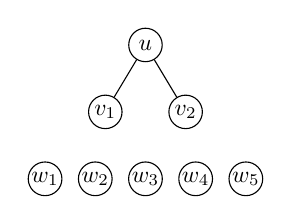
\begin{tikzpicture}[scale=0.85, every node/.style={scale=0.85,shape=circle,inner sep=.5pt,
                  minimum size=5mm}]
              \node[draw] (u) at (0,1) {$u$};
              \node[draw] (v1) at (-.6,0) {$v_1$};
              \node[draw] (v2) at (.6,0) {$v_2$};
              \node[draw] (w1) at (-1.5,-1) {$w_1$};
              \node[draw] (w2) at (-.75,-1) {$w_2$};
              \node[draw] (w3) at (0,-1) {$w_3$};
              \node[draw] (w4) at (.75,-1) {$w_4$};
              \node[draw] (w5) at (1.5,-1) {$w_5$};
              \draw (u) -- (v1);
              \draw (u) -- (v2);
          \end{tikzpicture}
        }
        \label{figure:gac-example-3}
    }
    \subfigure[][$H_2$] {
        \centering
        \scalebox{1}{
          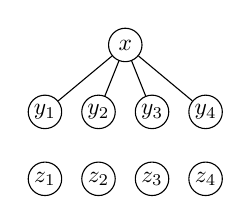
\begin{tikzpicture}[scale=0.85, every node/.style={scale=0.85,shape=circle,inner sep=.5pt,
                  minimum size=5mm}]
              \node[draw] (x) at (0,1) {$x$};
              \node[draw] (y1) at (-1.2,0) {$y_1$};
              \node[draw] (y2) at (-.4,0) {$y_2$};
              \node[draw] (y3) at (.4,0) {$y_3$};
              \node[draw] (y4) at (1.2,0) {$y_4$};
              \node[draw] (z1) at (-1.2,-1) {$z_1$};
              \node[draw] (z2) at (-.4,-1) {$z_2$};
              \node[draw] (z3) at (.4,-1) {$z_3$};
              \node[draw] (z4) at (1.2,-1) {$z_4$};
              \draw (x) -- (y1);
              \draw (x) -- (y2);
              \draw (x) -- (y3);
              \draw (x) -- (y4);
          \end{tikzpicture}
        }
        \label{figure:gac-example-4}
    }
    \subfigure[][$G_k$] {
        \centering
        \scalebox{1}{
          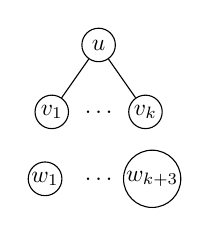
\begin{tikzpicture}[scale=0.85, every node/.style={scale=0.85,shape=circle,inner sep=.5pt,
                  minimum size=5mm}]
              \node[draw] (u) at (0,1) {$u$};
              \node[draw] (v1) at (-.7,0) {$v_1$};
              \node[] (vdots) at (0,0) {$\dots$};
              \node[draw] (v2) at (.7,0) {$v_k$};
              \node[draw] (w1) at (-.8,-1) {$w_1$};
              \node[] (wdots) at (0,-1) {$\dots$};
              \node[draw] (w5) at (.8,-1) {$w_{k+3}$};
              \draw (u) -- (v1);
              \draw (u) -- (v2);
          \end{tikzpicture}
        }
        \label{figure:gac-example-1}
    }
    \subfigure[][$H_k$] {
        \centering
        \scalebox{1}{
          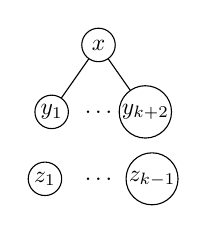
\begin{tikzpicture}[scale=0.85, every node/.style={scale=0.85,shape=circle,inner sep=.5pt,
                  minimum size=5mm}]
              \node[draw] (x) at (0,1) {$x$};
              \node[draw] (y1) at (-.7,0) {$y_1$};
              \node[] (ydots) at (0,0) {$\dots$};
              \node[draw] (y2) at (.7,0) {$y_{k+2}$};
              \node[draw] (z1) at (-.8,-1) {$z_1$};
              \node[] (zdots) at (0,-1) {$\dots$};
              \node[draw] (z5) at (.8,-1) {$z_{k-1}$};
              \draw (x) -- (y1);
              \draw (x) -- (y2);
          \end{tikzpicture}
        }
        \label{figure:gac-example-2}
    }
    \caption{Example graphs $G_2$ and $H_2$, and their generalised
    versions $G_k$ and $H_k$.}\label{figure:gac-example}
\end{figure}

When solving this instance, \McSplit-SI begins by mapping $u$ to $x$.  This leaves
two label classes:
$\langle \{v_1,v_2\}, \{y_1,y_2,y_3,y_4\} \rangle$
and
$\langle \{w_1,w_2,w_3,w_4,w_5\}, \{z_1,z_2,z_3,z_4\} \rangle$.  In the latter
label class, the first set of vertices is larger than the second, and therefore the
algorithm can backtrack and terminate.

Now we consider how the Glasgow algorithm behaves on this instance. After mapping
$u$ to $x$, the domains correspond to our label classes, as shown in the first
column of \Cref{tab:counting-all-diff}.  The remaining two columns of the table
illustrate the behaviour of the counting all-different propagator on these domains.
(Since all domains are of the same size, the stable sort function used by the algorithm
does not reorder the domains.)  The third column shows set $A$, which is the union
of domains in the current and previous rows.  The fourth column shows the number
of variables up to and including the current row.  Since $|A| \geq n$ on each row,
the propagator does not delete any values from the domains and does not conclude
that we can backtrack.

\begin{table}[h!]
\centering
\footnotesize
    \begin{tabular}{p{0.09\linewidth} p{0.16\linewidth} p{0.3\linewidth} p{0.08\linewidth}}
 \toprule
     Variable & Domain & $A$ & $n$\\ [0.5ex]
 \midrule
     $v_1$ & $\{y_1,y_2,y_3,y_4\}$ & $\{y_1,y_2,y_3,y_4\}$ & 1\\
     $v_2$ & $\{y_1,y_2,y_3,y_4\}$ & $\{y_1,y_2,y_3,y_4\}$ & 2\\
     $w_1$ & $\{z_1,z_2,z_3,z_4\}$ & $\{y_1,y_2,y_3,y_4,z_1,z_2,z_3,z_4\}$ & 3\\
     $w_2$ & $\{z_1,z_2,z_3,z_4\}$ & $\{y_1,y_2,y_3,y_4,z_1,z_2,z_3,z_4\}$ & 4\\
     $w_3$ & $\{z_1,z_2,z_3,z_4\}$ & $\{y_1,y_2,y_3,y_4,z_1,z_2,z_3,z_4\}$ & 5\\
     $w_4$ & $\{z_1,z_2,z_3,z_4\}$ & $\{y_1,y_2,y_3,y_4,z_1,z_2,z_3,z_4\}$ & 6\\
     $w_5$ & $\{z_1,z_2,z_3,z_4\}$ & $\{y_1,y_2,y_3,y_4,z_1,z_2,z_3,z_4\}$ & 7\\
%    $s_G$ & Pointer to Integer & Pointer to the first vertex of the $G$-set\\
%    \rule{0pt}{2.3ex}$e_G$ & Pointer to Integer & Pointer to one element past the last vertex of the $G$-set\\
 \bottomrule
\end{tabular}
\caption{A demonstration of the counting all-different propagator on $G_2$ and $H_2$
    after assigning $u$ to $x$.}
\label{tab:counting-all-diff}
\end{table}

The final two graphs in \Cref{fig:gac-example} generalise $G_2$ and $H_2$; as $k$ is incremented,
a vertex is added to each of the $v$, $w$, $y$ and $z$ sets.
\Cref{tab:gk-run-times} shows run times for the enumeration problem
using \McSplit-SI, Glasgow, and RI for a range of values of $k$.
VF3 was excluded because it reported incorrect results.
\McSplit-SI solves the instance $k=1\,000\,000$ in less than a second;
Glasgow and RI time out on the $k=10$ and $k=6$ instances respectively.

\begin{table}[h!]
\centering
\footnotesize
    \begin{tabular}{r r r r}
 \toprule
     $k$ & \McSplit-SI & Glasgow & RI \\ [0.5ex]
 \midrule
        3 & 0 & 0 & 2 \\
        4 & 0 & 0 & 84 \\
        5 & 0 & 2 & 3934 \\
        6 & 0 & 18 & * \\
        7 & 0 & 184 & * \\
        8 & 0 & 1849 & * \\
        9 & 0 & 21067 & * \\
        10 & 0 & * & * \\
        10000 & 5 & * & * \\
        100000 & 148 &  * & * \\
        1000000 & 584 & * & * \\
 \bottomrule
\end{tabular}
\caption{Run times in ms for the induced subgraph isomorphism enumeration problem on $G_k$.
    An asterisk indicates timeout at 30 seconds.}
\label{tab:gk-run-times}
\end{table}

\section{Conclusion}

We have introduced a version of McSplit for the induced subgraph isomorphism problem that is time- and memory-efficient for large, sparse graphs, and shown experimentally that it outperforms state-of-the-art algorithms on many instances.

Future work could use the data structures of McSplit-SI in the McSplit algorithm for maximum common induced subgraph.
